\section[class file format]{class file format}
这一节的内容来自\href{http://hxraid.iteye.com/blog/687660}{这个}网页和JVM Spec 8。

\subsection[整体布局]{整体布局}
class文件整体布局如图\ref{fig:dotclass}所示,具体数据结构如下(来自JVM Spec 8),

\begin{figure}
  \centering
  % Requires \usepackage{graphicx}
  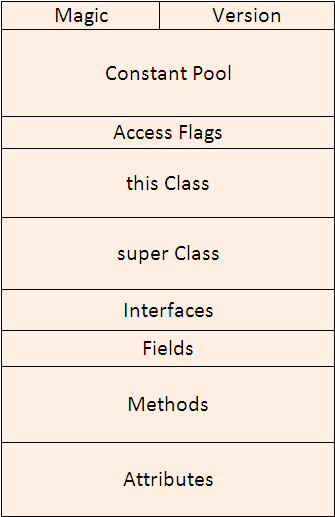
\includegraphics[width=.4\textwidth]{picturedir/JavaClassFileLayout.png}\\
  \caption{.class文件布局}\label{fig:dotclass}
\end{figure}

\begin{javacode}
ClassFile {
  u4 magic;
  u2 minor_version;
  u2 major_version;
  u2 constant_pool_count;
  cp_info constant_pool[constant_pool_count-1];
  u2 access_flags;
  u2 this_class;
  u2 super_class;
  u2 interfaces_count;
  u2 interfaces[interfaces_count];
  u2 fields_count;
  field_info fields[fields_count];
  u2 methods_count;
  method_info methods[methods_count];
  u2 attributes_count;
  attribute_info attributes[attributes_count];
}
\end{javacode}

进一步,各种info数据结构,

\begin{javacode}
cp_info {
  u1 tag;
  u1 info[];
}

field_info {
  u2 access_flags;
  u2 name_index;
  u2 descriptor_index;
  u2 attributes_count;
  attribute_info attributes[attributes_count];
}

method_info {
  u2 access_flags;
  u2 name_index;
  u2 descriptor_index;
  u2 attributes_count;
  attribute_info attributes[attributes_count];
}

attribute_info {
  u2 attribute_name_index;
  u4 attribute_length;
  u1 info[attribute_length];
}
\end{javacode}

class文件由8比特的字节流组成,全部字节流构成15个有意义的条目。
\begin{enumerate}
  \item magic number,0xCAFEBABE,表明一个文件是.class文件
  \item minor version, major version,主次版本号
  \item constant pool count,常量池大小
  \item constant pool,大小不固定,常量池,详见\ref{sec:constantpool}节
  \item access flag,表明类/接口、访问修饰符、是否抽象类、是否final类
  \item this class,它是一个常量池索引
  \item super class,它是一个常量池索引
  \item interface count, interface,接口数量以及接口的具体信息
  \item fields count, fields,属性的数量及其具体信息
  \item method count, methods,方法的数量及其具体信息(包括方法的实现)
\end{enumerate}

\subsection[常量池]{常量池}
\label{sec:constantpool}
常量池是由一个个item组成,就像一个表格,所有item总共有如下不同的类型,
每一种类型都由一个tag(1字节的常数)来标识,各种不同类型的数据结构定义
如下(来自JVM Spec 8,另外还有几种增加的类型没有列出),

\begin{javacode}
// 除了基本类型和UTF8类型存在“实际”数据以外,其他都是保存index而已!
CONSTANT_Class_info {
  u1 tag;
  u2 name_index;
}
CONSTANT_Fieldref_info {
  u1 tag;
  u2 class_index;
  u2 name_and_type_index;
}
CONSTANT_Methodref_info {
  u1 tag;
  u2 class_index;
  u2 name_and_type_index;
}
CONSTANT_InterfaceMethodref_info {
  u1 tag;
  u2 class_index;
  u2 name_and_type_index;
}
CONSTANT_String_info {
  u1 tag;
  u2 string_index;
}
CONSTANT_Integer_info {
  u1 tag;
  u4 bytes; // int占4个字节
}
CONSTANT_Float_info {
  u1 tag;
  u4 bytes; // float占4个字节
}
CONSTANT_Long_info {
  u1 tag;
  u4 high_bytes; // long占8个字节
  u4 low_bytes;
}
CONSTANT_Double_info {
  u1 tag;
  u4 high_bytes; // double占8个字节
  u4 low_bytes;
}
CONSTANT_NameAndType_info {
  u1 tag;
  u2 name_index;
  u2 descriptor_index;
}
CONSTANT_Utf8_info {
  u1 tag;
  u2 length;
  u1 bytes[length]; // 所有的“符号”都以UTF8形式存在
}
\end{javacode}

这些类型的tag值如表\ref{tab:constantpooltype}所示。

\begin{table}
\centering
\begin{tabular}{r|c|l}
Type & Flag\newline(1 byte) & Format \\
\hline\hline
CONSTANT\_Utf8 & 1 & <flag> <length> <data>\\
CONSTANT\_Integer & 3 & <flag> <data>\\
CONSTANT\_Float & 4 & <flag> <data>\\
CONSTANT\_Long & 5 & <flag> <data>\\
CONSTANT\_Double & 6 & <flag> <data>\\
CONSTANT\_Class & 7 & <flag> <index>\\
CONSTANT\_String & 8 & <flag> <index>\\
CONSTANT\_Fieldref & 9 & <flag> <index>\\
CONSTANT\_Methodref & 10 & <flag> <index>\\
CONSTANT\_InterfaceMethodref & 11 & <flag> <index>\\
CONSTANT\_NameAndType & 12 & <flag> <index>\\
\hline
\end{tabular}
\caption{Constant Pool format}\label{tab:constantpooltype}
\end{table}

需要注意的是真正数据存在于各种基本类型以及UTF8类型中,
其他的索引最终都要落到某个UTF8的数据处,这些数据即为
“符号”,如类的全限定名称,方法的完整签名等,运行时的
“符号解析”解析的就是这里的符号,其实就是一些字符串而已。

\subsection[实例解析]{实例解析}
以如下代码编译出来的class文件,逐个字节分析。

\begin{javacode}
package hr.test;
public class ClassTest {
  private int itemI = 0;
  private static String itemS = "我们";
  private final float PI = 3.1415926F;

  public ClassTest() { }

  public int getItemI() {
    return this.itemI;
  }

  public static String getItemS() {
    return itemS;
  }

  public static void main(String[] args) {
    ClassTest ct = new ClassTest();
  }
}
\end{javacode}

下面是逐字节分析,每个字节翻译为十进制数字。

%\input{srcdir/analyse.txt}

\begin{description}
\item[magic number:] 202 254 186 190
\item[minor version:] 0 0
\item[major version:] 0 50
\item[constant pool:] 0 43 常量池的长度,index从1开始,0被保留
	\begin{enumerate}
	\item 7 0 2\\
		对类ClassTest的符号引用(7为标志  02指向了常量池的索引2的位置)
	\item 1 0 17 104 114 47 116 101 115 116 47 67 108 97 115 115 84 101 115 116\\
		类全限定名"hr\bs test\bs ClassTest"
	\item 7 0 4\\
		对类Object的符号引用
	\item 1 0 16 106 97 118 97 47 108 97 110 103 47 79 98 106 101 99 116\\
		超类全限定名"java/lang/Object"
	\item 1 0 5 105 116 101 109 73\\
		第1个类字段名"itemI"
	\item 1 0 1 73\\
		第1个类字段类型为整型'I'
	\item 1 0 5 105 116 101 109 83\\
		第2个类字段名"itemS"
	\item 1 0 18 76 106 97 118 97 47 108 97 110 103 47 83 116 114 105 110 103 59\\
		第2个类字段类型的全限定名"Ljava/lang/String"
	\item 1 0 2 80 73\\
		第3个类字段名"PI"
	\item 1 0 1 70\\
		第3个类字段类型为'F'
	\item 1 0 13 67 111 110 115 116 97 110 116 86 97 108 117 101\\
		第3个类字段为常量"ConstantValue"
	\item 4 64 73 15 218\\
		第3个类字段float字面值,占4bytes(3.1415926)
	\item 1 0 8 60 99 108 105 110 105 116 62\\
		初始化方法名"<clinit>"
	\item 1 0 3 40 41 86\\
		方法的返回类型为"()V",即void
	\item 1 0 4 67 111 100 101\\
		"Code"
	\item 8 0 17\\
		String字符串字面值(0 17表示索引17)
	\item 1 0 6 230 136 145 228 187 172\\
		"我们"
	\item 9 0 1 0 19\\
		指向第2个字段的引用(0 1指向索引1,0 19指向索引19)
	\item 12 0 7 0 8\\
		指向第2个字段的名字和描述符的索引,
	\item 1 0 15 76 105 110 101 78 117 109 98 101 114 84 97 98 108 101\\
		"LineNumberTable"
	\item 0 18 76 111 99 97 108 86 97 114 105 97 98 108 101 84 97 98 108 101\\
		"LocalVariableTable"
	\item 1 0 6 60 105 110 105 116 62\\
		表示初始化方法名"<init>"
	\item 10 0 3 0 24\\
		指向父类Object的构造器方法,0 3表示父类名常量表的索引,0 24表示存放该方法名称和描述符的引用的常量表的索引
	\item 12 0 22 0 14\\
		指向方法名和描述符的常量表的索引。0 22是方法名的常量表索引,0 14是描述符的常量表索引
	\item 9 0 1 0 26\\
		指向第1个字段的引用, 0 1表示字段所属类型的索引,0 26表示字段名和描述符的索引
	\item 12 0 5 0 6\\
		指向第1个字段的名字和描述符的索引
	\item 9 0 1 0 28\\
		指向第3个字段的引用, 0 1表示字段所属类型的索引,0 28表示字段名和描述符的索引
	\item 12 0 9 0 10\\
		指向第3个字段的名字和描述符的索引
	\item 1 0 4 116 104 105 115\\
		隐含参数符号"this"
	\item 1 0 11 76 67 108 97 115 115 84 101 115 116 59\\
		"LClassTest;"
	\item 1 0 8 103 101 116 73 116 101 109 73\\
		方法名"getItemI"
	\item 1 0 3 40 41 73\\
		方法描述符"()I",即返回类型为int
	\item 1 0 8 103 101 116 73 116 101 109 83\\
		方法名"getItemS"
	\item 1 0 20 40 41 76 106 97 118 97 47 108 97 110 103 47 83 116 114 105 110 103 59\\
		方法描述符"()Ljava/lang/String;"
	\item 1 0 4 109 97 105 110\\
		主方法名"main"
	\item 1 0 22 40 91 76 106 97 118 97 47 108 97 110 103 47 83 116 114 105 110 103 59 41 86\\
		主方法中的参数的字符串数组类型名"()Ljava/lang/String;)V"
	\item 10 0 1 0 24\\
		指向当前 ClassTest 类的构造器方法,0 1表示存放当前类名的常量表的索引。0 24是存放方法名和描述符的符号引用的常量表索引。
	\item 1 0 4 97 114 103 115\\
		参数"args"
	\item 1 0 19 91 76 106 97 118 97 47 108 97 110 103 47 83 116 114 105 110 103 59\\
		字符串数组"[Ljava/lang/String;"
	\item 1 0 2 99 116\\
		对象符号"ct"
	\item 1 0 10 83 111 117 114 99 101 70 105 108 101\\
		"SourceFile"
	\item 1 0 14 67 108 97 115 115 84 101 115 116 46 106 97 118 97\\
		"ClassTest.java"
	\end{enumerate}
\item [access flags:] 0 33 访问标志:public
\item [this Class:] 0 1 指向当前类的符号引用在常量池中的索引
\item [super Class:] 0 3 指向当前类的父类的符号引用在常量池中的索引
\item [inteface count:] 0 0 接口的数量
\item [field count:] 0 3 字段的数量
\item [fields:] fields的具体内容
	\begin{enumerate}
	\item 字段 itemI\\
		0 2  --- private 修饰符\\
		0 5  --- 字段名在常量池中的索引,字段itemI\\
		0 6  --- 字段的描述符(所属类型)在常量池中的索引\\
		0 0  --- 字段的属性信息表(attribute\_info)的数量
	\item 字段 itemS\\
		0 10 ---- private static 修饰符\\
		0 7  --- 字段名在常量池中的索引,字段itemS\\
		0 8  --- 字段的描述符(所属类型)在常量池中的索引\\
		0 0  --- 字段的属性信息表(attribute\_info)的数量
	\item 字段 PI\\
		0 18 --- private final 修饰符\\
		0 9  --- 字段名在常量池中的索引,//字段PI\\
		0 10 --- 字段的描述符(所属类型)在常量池中的索引\\
		0 1  --- 字段的属性信息表(attribute\_info)的数量\\
		0 11 --- 属性名在常量池中的索引。即ConstantValue\\
		0 0 0 2 --- 属性所占的字节长度\\
		0 12 --- 属性值在常量池中的索引。即常量字面值
	\end{enumerate}
\item [method count:] 0 5 方法的数量
\item [methods:] methods的内容
	\begin{enumerate}
	\item 类的静态数据初始化方法<clinit>\\
		0 8  --- static 修饰符(所有的初始化方法都是static的)\\
		0 13 --- 在常量池中的索引。初始化方法名<clinit>,该方法直接由JVM在特定的时候调用,并非由字节码生成。\\
		0 14 --- 在常量池中的索引。返回类型为void。\\
		0 1  --- 属性数量\\
		0 15 --- 属性名 在常量池中的索引。即code\\
		0 0 0 42 ---  属性所占的字节长度42\\
		0 1 0 0 0 0 0 6 18 16 179 0 18 177 0 0 0 2 0 20 0 0 0 10 0 2 0 0 0 5 0 5 0 2 0 21 0 0 0 2 0 0 --- 该方法的字节码指令序列和其他信息
	\item 类的普通实例数据的初始化方法,针对类构造器生成的<init>方法。\\
		0 1  --- public 修饰符\\
		0 22 --- 构初始化方法名<init>\\
		0 14 --- 构造器的返回类型为void\\
		0 1  --- 属性数量\\
		0 15 ---  属性名在常量池中的索引。即Code\\
		0 0 0 70 -- 属性所占的字节长度70\\
		0 2 0 1 0 0 0 16 42 183 0 23 42 3 181 0 25 42 18 12 181 0 27 177 0 0 0 2 0 200 0 0 18 0 4 0 0 0 8 0 4 0 4 0 9 0 6 0 15 0 9 0 21 0 0 0 12 0 10 0 0 16 0 29 0 30 0 0
		---	该方法的字节码指令序列和其他信息
	\item getItemI方法\\
		0 1  --- public 修饰符\\
		0 31 --- 在常量池中的索引。方法名getItemI\\
		0 32 --- 在常量池中的索引。方法返回类型为int\\
		0 1  --- 属性数量\\
		0 15 --- 属性名在常量池中的索引。即Code\\
		0 0 0 47 ---  属性所占的字节长度70\\
		0 1 0 1 0 0 0 5 42 180 0 25 172 0 0 0 2 0 20 0 0 0 6 0 1 0 0 0 12 0 21 0 0 0 12 0 1 0 0 0 5 0 29 0 30 0 0 --- 该方法的字节码指令序列和其他信息
	\item getItemS方法\\
		0 9  --- public static 修饰符\\
		0 33 --- 在常量池中的索引。方法名getItemS\\
		0 34 --- 在常量池中的索引。方法返回类型为String\\
		0 1  --- 属性数量\\
		0 15 --- 属性名在常量池中的索引。即Code\\
		0 0 0 36 ---  属性所占的字节长度36\\
		0 1 0 0 0 0 0 4 178 0 18 176 0 0 0 2 0 20 0 0 0 6 0 1 0 0 0 16 0 21 0 0 0 2 0 0 --- 该方法的字节码指令序列和其他信息
	\item main方法\\
		0 9  --- public static 修饰符\\
		0 35 ---  在常量池中的索引。主方法名main\\
		0 36 --- 在常量池中的索引。方法返回类型为String[]\\
		0 1  --- 属性数量\\
		0 15 ---  属性名在常量池中的索引。即Code\\
		0 0 0 65 --- 属性所占的字节长度36\\
		0 2 0 2 0 0 0 9 187 0 1 89 183 0 37 76 177 0 0 0 2 0 20 0 0 0 10 0 2 0 0 0 20 0 8 0 21 0 21 0 0 0 22 0 2 0 0 0 9 0 38 0 39 0 0 0 8 0 1 0 40 0 30 0 1 0 1 0 41 0 0 0 2 0 42
		--- 该方法的字节码指令序列和其他信息
	\end{enumerate}
\end{description}
